%! Author = Len Washington III
%! Date = 9/16/24

% Preamble
\documentclass[
	chapter=4
]{chem122notes}
\usepackage{cancel}

% Packages

% Document
\begin{document}

\section{Outline}\label{sec:outline}
\begin{itemize}
	\item Aqueous solutions (electrolytes, concentrations)
	\item Precipitation reactions (soluble and insoluble compounds)
	\item Molecular, ionic, and net ionic equations
	\item Oxidation-Reduction reactions
\end{itemize}

\section{Terminology}\label{sec:terminology}
In \emph{solutions}, we need to define the following terms:
\begin{itemize}
	\item \definition{solvent}{The medium (e.g., water, ethanol, benzene, etc.) in which a solute is dissolved to form a solution.}
	\item \definition{solute}{The substance (e.g. NaCl, glucose, etc.) dissolved in a solvent to form a solution.}
\end{itemize}

\section{Concentration of Solute}\label{sec:concentration-of-solute}
The amount of solute in a solution is given by its \emph{concentration}.
\begin{equation}
	\mbox{Molarity(M)} = \frac{\mbox{moles of solute}}{\mbox{liters of solution}}
	\label{eq:molarity}
\end{equation}

\begin{equation*}
\begin{aligned}
	[\mbox{NaCl}] &= 0.1 M\\
		      &= \frac{0.1 \mbox{ moles of NaCl}}{1 \mbox{ L of solution}}
\end{aligned}
\end{equation*}

\section{Preparing Solutions}\label{sec:preparing-solutions}
\begin{itemize}
	\item Weigh out a solid solute and dissolve in a given quantity of solvent.
	\item \emph{Dilute} a concentrated solution to give one that is less concentrated.
\end{itemize}

\section{Using Molarity}\label{sec:using-molarity}
What mass of oxalic acid, $\chemical{H}[2]\chemical{C}[2]\chemical{O}[4]$, is required to make 250.00 mL of a 0.0500 M solution?

\begin{equation*}
\begin{aligned}
	\mbox{molar mass} &= (2*1.008) + (2*12.011) + (4 * 15.999)\\
			  &= 2.016 + 24.022 + 63.996\\
			  &= 90.034 \mbox{ g mol}^{-1}\\
\end{aligned}
\end{equation*}
\begin{equation*}
\begin{aligned}
	250.00 \mbox{ mL} \times \frac{1 \mbox{ L}}{1,000 \mbox{ mL}} \times \frac{0.05 \mbox{ mol}}{1 \mbox{L}} \times \frac{90.034 \mbox{ g }\chemical{H}[2]\chemical{C}[2]\chemical{O}[4]}{1 \mbox{ mol } \chemical{H}[2]\chemical{C}[2]\chemical{O}[4]} = 1.125425 \mbox{ g }\chemical{H}[2]\chemical{C}[2]\chemical{O}[4]\\
\end{aligned}
\end{equation*}

\section{Preparing a Solution by Dilution}\label{sec:preparing-a-solution-by-dilution}
You have 50.0 mL of 3.0 M NaOH and you want 0.50 M NaOH\@.
What does one do?

\begin{equation*}
\begin{aligned}
	M_{1}V_{1} &= M_{2}V_{2}\\
	(3.0)(50.0) &= (0.5)V_{2}\\
	V_{2} &= \frac{(3.0)(50.0)}{0.5}\\
	V_{2} &= (6.0)(50.0)\\
	V_{2} &= 300.0\mbox{ mL}\\
		  &= 3.0\times10^{2}\mbox{ mL}
\end{aligned}
\end{equation*}

In an acid-base titration, it takes 38.55 mL of 0.650 M perchloric acid (HCl$\chemical{O}[4]$) to completely neutralize 25.00 mol calcium hydroxide ($\chemical{Ca}(\chemical{O}\chemical{H}[2])$) solution.
\[ \chemical{Ca}(\chemical{O}\chemical{H}[2]) (\mbox{aq.}) + 2\chemical{H}\chemical{Cl}\chemical{O}[4] (\mbox{aq.}) \rightarrow \chemical{Ca}( \chemical{Cl}{O_{4}} )_{2} (\mbox{aq.}) + 2\chemical{H}[2]\chemical{O} (\mbox{l}) \]
\begin{enumerate}[label=\Alph*)]
	\item How many moles of $\chemical{H}\chemical{Cl}\chemical{O}[4]$ are needed for the complete neutralization?
	\begin{equation*}
	\begin{aligned}
		38.55\mbox{mL perchloric acid} \times \frac{1 \mbox{ L perchloric acid}}{1,000 \mbox{ mL perchloric acid}} \times \frac{0.650 \mbox{ mol}}{1 \mbox{ L}} = 0.0251 \mbox{ mol perchloric acid}
	\end{aligned}
	\end{equation*}
	\item How many moles of $\chemical{Ca}(\chemical{O}\chemical{H}[2])_{2}$ got consumed during the neutralization?
	\begin{equation*}
	\begin{aligned}
		0.0251 \mbox{ mol perchloric acid} \times \frac{1 \mbox{ mol } \element{Ca}(\element{O}\element{H}[2])_{2}}{2 \mbox{ mol perchloric acid}} &= 0.01255 \ \element{Ca}(\element{O}\element{H}[2])_{2}
	\end{aligned}
	\end{equation*}
	\item What is the concentration of $\element{Ca}(\element{O}\element{H}[2])_{2}$ in the original solution before titration?
	\begin{equation*}
	\begin{aligned}
		\frac{25.00 \mbox{ mol } \element{Ca}(\element{O}\element{H}[2])_{2}}{38.55 \mbox{mL}} \times \frac{1,000 \mbox{ mL}}{1 \mbox{ mL}} =
	\end{aligned}
	\end{equation*}
\end{enumerate}

\section{Dissociation}\label{sec:dissociation}
\begin{itemize}
	\item When an ionic compound dissolves in water, the solvent pulls the individual ions from the crystal and solvates them.
	\item This process is called \emph{dissociation}.
\end{itemize}
\[ \element{Na}\element{Cl} (\mbox{s}) \rightarrow \element{Na}^{+} (\mbox{aq}) + \element{Cl}^{-}(\mbox{aq}) \]
\begin{itemize}
	\item An \emph{electrolyte} is a substance that dissociates into ions when dissolved in water.
	\item Ionic compounds dissociate in water (e.g., NaCl, $\element{Ba}{Cl}[2]$, etc.)
	\item Only a few molecular compounds are capable of dissociating in water.
	\item For example, \[ \chemical{H}\chemical{Cl} (\mbox{aq.}) \rightarrow \chemical{H}^{+} (\mbox{aq.}) + \chemical{Cl}^{-} (\mbox{aq.}) \]
\end{itemize}

\section{Electrolytes}\label{sec:electrolytes}
\begin{itemize}
	\item An \emph{electrolyte} is a substance that dissociates into ions when dissolved in water.
	\item A \emph{nonelectrolyte} may dissolve in water, but it does not dissociate into ions when it does so.
	\item There are many examples of molecular compounds (e.g., methanol ($\element{C}\element{H}[3]\element{OH}$), table sugar (sucrose; $\element{C}[12]\element{H}[12]\element{O}[11]$)) that serve as nonelectrolytes in water.
\end{itemize}

\begin{table}[H]
	\centering
	\caption{Summary}
	\label{tab:electrolyte-bonds}
	\begin{tabular}{l l l l}
		& \textbf{Strong Electrolyte} & \textbf{Weak Electrolyte} & \textbf{Nonelectrolyte}\\
		\hline
		\textbf{Ionic} & All & None & None\\
		\textbf{Molecular} & Strong acids (see Table 4.2) & Weak acids & \\
		& & Weak bases & All other compounds\\
		\hline
	\end{tabular}
\end{table}
e.g., the molecular compound HCl is a strong acid that dissociates completely in water.
As a result, HCl is a strong electrolyte.
\[ \chemical{H}\chemical{Cl} (\mbox{aq.}) \rightarrow \chemical{H}^{+} (\mbox{aq.}) + \chemical{Cl}^{-} (\mbox{aq.}) \]
e.g., the molecular compound acetic acid, $\element{C}\element{H}[3]\element{C}\element{O}\element{O}\element{H}$, is a weak acid that is only partially dissociated.
As a result, acetic acid is a weak electrolyte.
\[ \element{C}\element{H}[3]\element{C}\element{O}\element{O}\element{H} (\mbox{aq.}) \leftrightarrow \element{C}\element{H}[3]\element{C}\element{O}\element{O}^{-} (\mbox{aq.}) + \element{H}^{+} (\mbox{aq.}) \]

\begin{itemize}
	\item Ion concentration can be measured using conductivity.
	Ions carry electrical charge from one electrode to the other, completing the electrical circuit.
	\begin{description}
		\item[No ions] A nonelectrolyte solution does not contain ions, and the bulb does not light.
		\item[Few ions] If the solution contains a small number of ions, the bulb will by only dimly lit.
		\item[Many ions] If the solution contains a large number of ions, the bulb will be brightly lit.
	\end{description}
\end{itemize}

\section{Strong Electrolytes Are$\dots$}\label{sec:strong-electrolytes-are}
\begin{itemize}
	\item Strong acids
	\begin{description}
		\item[HCl] Hydrochloric
		\item[HBr] Hydrobromic
		\item[HI] Hydroiodic
		\item[HCl$\mbox{O}_{3}$] Chloric
		\item[HCl$\mbox{O}_{4}$] Perchloric
		\item[HN$\mbox{O}_{3}$] Nitric
		\item[$\mbox{H}_{2}\mbox{SO}_{4}$] Sulfuric
	\end{description}
	\item Strong bases
	\begin{itemize}
		\item Group 1A metal hydroxides
		\begin{itemize}
			\item LiOH
			\item NaOH
			\item KOH
			\item RbOH
			\item CsOH
		\end{itemize}
		\item Heavy group 2A metal hydroxides
		\begin{itemize}
			\item $\element{Ca}(\element{OH})_{2}$
			\item $\element{Sr}(\element{OH})_{2}$
			\item $\element{Ba}(\element{OH})_{2}$
		\end{itemize}
	\end{itemize}
	\item Also soluble ionic salts
\end{itemize}
\begin{table}[H]
	\centering
	\caption{Solubility Guidelines for Common Ionic Compounds in Water}
	\label{tab:ionic-compound-solubility-guidelines}
	\begin{tabular}{l l l}
		\textbf{Soluble Ionic Compounds} & & \textbf{Important Exceptions}\\
		\hline
		Compounds containing & $\chemical{N}\chemical{O}_{3}^{-}$ & None\\
		 & $\element{C}\element{H}[3]\element{C}\element{O}\element{O}^{-}$ & None\\
		 & $\element{Cl}^{-}$ & Compounds of $\element{Ag}^{+},\ \element{Hg}[2]^{2+}$, and $\element{Pb}^{2+}$\\
		 & $\element{Br}^{-}$ & Compounds of $\element{Ag}^{+},\ \element{Hg}[2]^{2+}$, and $\element{Pb}^{2+}$\\
		 & $\element{I}^{-}$ & Compounds of $\element{Ag}^{+},\ \element{Hg}[2]^{2+}$, and $\element{Pb}^{2+}$\\
		 & $\element{S}\element{O}[4]^{2-}$ & Compounds of $\element{Sr}^{2+}, \element{Ba}^{2+}, \element{Hg}[2]^{2+}$, and $\element{Pb}^{2+}$\\
		\hline
		\textbf{Insoluble Ionic Compounds} & & \textbf{Important Exceptions}\\
		\hline
		Compounds containing & $\element{S}^{2-}$ & Compounds of $\element{N}\element{H}_{4}^{+}$, the alkali metal cations, $\element{Ca}^{2+},\ \element{Sr}^{2+}$, and $\element{Ba}^{2+}$\\
		& $\element{C}\element{O}[3]^{2-}$ & Compounds of $\element{N}\element{H}_{4}^{+}$ and the alkali metal cations\\
		& $\element{P}\element{O}[4]^{3-}$ & Compounds of $\element{N}\element{H}_{4}^{+}$ and the alkali metal cations\\
		& $\element{O}\element{H}^{-}$ & Compounds of $\element{N}\element{H}_{4}^{+}$, the alkali metal cations, $\element{Ca}^{2+},\ \element{Sr}^{2+}$, and $\element{Ba}^{2+}$\\
		\hline % TODO: Set column widths
	\end{tabular}
\end{table}
\begin{itemize}
	\item \emph{Note that all common ionic compounds of the alkali metal ions (group 1A of the periodic table) and the ammonium ion ($\element{N}\element{H}_{4}^{+}$) are soluble in water.}
\end{itemize}

\section{Precipitation Reactions}\label{sec:precipitation-reactions}
When ions that are insoluble (as could be predicted by the solubility guidelines in Table~\ref{tab:ionic-compound-solubility-guidelines}) are mixed and form compounds, a \emph{precipitate} is formed.\\

\begin{minipage}[m]{0.6\textwidth}
	The insoluble yellow solid formed on the right is lead iodide ($\element{Pb}{I}[2]$).
	\[ 2\element{K}\element{I} (\mbox{aq}) + \element{Pb}(\element{N}\element{O}_{3})_{2} (\mbox{aq}) \rightarrow \element{Pb}\element{I}_{2} (\mbox{s}) + 2\element{K}\element{N}\element{O}[3] (\mbox{aq}) \]
\end{minipage}\hfill%
\begin{minipage}[t]{0.4\textwidth}
	\begin{figure}[H]
		\centering
		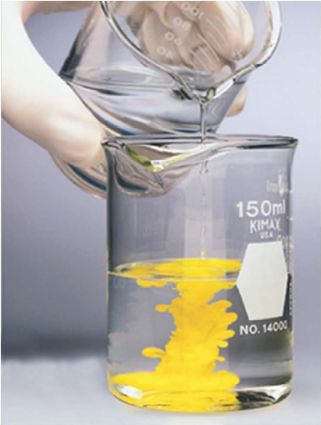
\includegraphics[width=\textwidth]{chapter4/lead_iodide}
		\caption{Lead Iodide}
		\label{fig:lead-iodide}
	\end{figure}
\end{minipage}

\section{Metathesis (Exchange) Reactions}\label{sec:metathesis-(exchange)-reactions}
\begin{itemize}
	\item Metathesis comes from a Greek word that means ``to transpose.''
	\item It appears that the ions in the reactants exchange, or transpose, ions.
	\item This is like switching dance partners!
	\[ \textcolor{blue}{\element{Ag}}\element{N}\element{O}[3] (\mbox{aq}) + \element{K}\textcolor{blue}{\element{Cl}} (\mbox{aq}) \leftrightarrow \textcolor{blue}{\element{Ag}\element{Cl}} (\mbox{s}) + \element{K}\element{N}\element{O}[3] (\mbox{aq}) \]
\end{itemize}

\section{Molecular Equation}\label{sec:molecular-equation}
The molecular equation lists the reactants and products in their molecular forms.
\[ \element{Ag}\element{N}\element{O}[3] (\mbox{aq}) + \element{K}\element{Cl} (\mbox{aq}) \leftrightarrow \element{Ag}\element{Cl} (\mbox{s}) + \element{K}\element{N}\element{O}[3] (\mbox{aq}) \]

\section{Ionic Equation}\label{sec:ionic-equation}
\begin{itemize}
	\item In the ionic equation, all strong electrolytes (strong acids, strong bases, and soluble ionic salts) are dissociated into their ions.
	\item This more accurately reflects the species that are found in the reaction mixture.
\end{itemize}

\begin{equation*}
\begin{aligned}
	\element{Ag}^{+} (\mbox{aq}) + \element{N}\element{O}[3]^{-} (\mbox{aq}) + \element{K}^{+} (\mbox{aq}) + \element{Cl}^{-} \rightarrow\\
	\element{Ag}\element{Cl} (\mbox{s}) + \element{K}^{+} (\mbox{aq}) + \element{N}\element{O}[3]^{-} (\mbox{aq})\\
\end{aligned}
\end{equation*}

\section{Net Ionic Equation}\label{sec:net-ionic-equation}
\begin{itemize}
	\item To form the net ionic equation, cross out anything that does not change from the left side of the equation to the right.
\end{itemize}
\begin{equation*}
	\begin{aligned}
		\element{Ag}^{+} (\mbox{aq}) + \cancel{\element{N}\element{O}[3]^{-} (\mbox{aq})} + \cancel{\element{K}^{+} (\mbox{aq})} + \element{Cl}^{-}\rightarrow\\
		\element{Ag}\element{Cl} (\mbox{s}) + \cancel{\element{K}^{+} (\mbox{aq})} + \cancel{\element{N}\element{O}[3]^{-} (\mbox{aq})}\\
	\end{aligned}
\end{equation*}
\begin{itemize}
	\item The only things left in the equation are those things that change (i.e., react) during the course of the reaction.
\end{itemize}
\begin{equation*}
	\begin{aligned}
		\element{Ag}^{+} (\mbox{aq}) + \element{Cl}^{-}\ \ \ \ \ \element{Ag}\element{Cl} (\mbox{s})
	\end{aligned}
\end{equation*}

\section{Oxidation-Reduction Reactions}\label{sec:oxidation-reduction-reactions}
\begin{itemize}
	\item An \emph{oxidation} occurs when at atom or ion \textit{loses} electrons.
	\item A \emph{reduction} occurs when an atom or ion \textit{gains} electrons.
	\item One cannot occur without the other.
\end{itemize}

\begin{figure}[H]
	\centering
	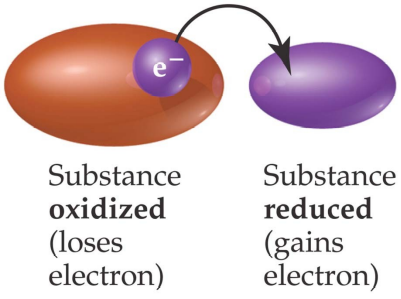
\includegraphics[width=0.5\textwidth]{chapter4/oxidation-reduction}
	\caption{Oxidation-Reduction Reactions}
	\label{fig:oxidation-reduction}
\end{figure}

\section{Oxidation Numbers}\label{sec:oxidation-numbers}
\begin{itemize}
	\item Elements in their elemental form have an oxidation number of 0.
	\item The oxidation number of a monatomic ion is the same as its charge.
	\item Nonmetals tend to have negative oxidation numbers, although some are positive in certain compounds or ions.
	\item Oxygen has an oxidation number of $-2$, except in the peroxide ion in which it has an oxidation number of $-1$.
	\item Hydrogen is $-1$ when bonded to a metal, $+1$ when bonded to a nonmetal.
	\item Fluorine always has an oxidation number of $-1$.
	\item The other halogens have an oxidation number of $-1$ when they are negative; they can have positive oxidation numbers; however, most notably in oxyanions (e.g., $\element{Cl}\element{O}[4]^{-}$).
	\item The sum of the oxidation numbers in a neutral compound is 0.
	\item The sum of the oxidation numbers in a polyatomic ion is the charge on the ion.
\end{itemize}

\section{Acids and Bases}\label{sec:acids-and-bases}
There are 3 definitions of acids and bases:
\begin{itemize}
	\item Arrhenius
	\item Br\o{}nsted
	\item Lewis
\end{itemize}
The original one was Arrhenius.
This describes the strong acids and bases, which was all they knew of at the time.

\subsection{Arrhenius}\label{subsec:arrhenius}
Acids contain $\element{H}^{+}$, bases contain $\element{OH}^{-}$.
This worked well until it was found that $\element{N}\element{H}[3]$ was a base - but no $\element{O}\element{H}^{-}$ in sight.
So $\dots$ redefine bases.

\subsection{Br\o{}nsted}\label{subsec:bronsted}
Acids are $\element{H}^{+}$ donors, bases are $\element{H}^{+}$ acceptors.
So acids have stayed essentially the same, but bases are now defined by the way they interact with acids.
Acid base reactions are now seen as the transfer of an $\element{H}^{+}$ ion.
\begin{equation*}
\begin{aligned}
	&\element{H}\element{Cl}& +\ &\element{N}\element{H}[3]& \rightarrow \element{N}\element{H}[4]^{+} + \element{Cl}^{-}\\
	&acid& &base&
\end{aligned}
\end{equation*}

This also means that acids and bases come in pairs, called conjugate pairs.
% TODO: Insert this drawing

Notice that the two conjugates differ by an $\element{H}^{+}$ ion.
\[ \element{N}\element{H}[3]\ \&\ \element{N}\element{H}[4]^{+}\ \ \ \ \element{H}\element{Cl}\ \&\ \element{Cl}^{-} \]

Some chemicals can act as both an acid \& a base -- we call them amphoteric.
For example:
% TODO: Insert this drawing too

The Br\o{}nsted definition works for most acid-base reactions, so to predict the products of an acid-base reaction, you transfer an $\element{H}^{+}$ from one chemical (the acid) to another (the base).
% TODO: And this one

And then $\dots$ the found acids that do not contain $\element{H}^{+}$, like $\element{Al}{Cl}[3]$.

\subsection{Lewis definition}\label{subsec:lewis-definition}
It seemed reasonable that acid-base chemistry should be described by electrons, all other reactions are.
So $\dots$
\begin{description}
	\item[Lewis acid] $\mbox{e}^{-}$ pair acceptor
	\item[Lewis base] $\mbox{e}^{-}$ pair donor
\end{description}
Notice that all the bases we have seen before have lone pairs of $\mbox{e}^{-}$.
When you draw the Lewis structure

% TODO: Insert drawing
So things that are only Lewis acids are those with empty orbitals, metal cations ($\element{Fe}^{2+}, \element{Cu}^{+}$) and Group 13 elements (Al, B, etc.)

These three definitions are a hierarchy.
All Arrhenius acids are also Br\o{}nsted acids and Lewis acids.
But not all Lewis acids are Br\o{}nsted and/or Arrhenius acids;
the same is true for bases.

\end{document}
